%!TEX root = minta_dolgozat.tex
%%%%%%%%%%%%%%%%%%%%%%%%%%%%%%%%%%%%%%%%%%%%%%%%%%%%%%%%%%%%%%%%%%%%%%%
\chapter{Neurális hálók}\label{ch:INTRO}
%%%%%%%%%%%%%%%%%%%%%%%%%%%%%%%%%%%%%%%%%%%%%%%%%%%%%%%%%%%%%%%%%%%%%%%
\section{Bevezető}
\subsection{Biológiai modell}

Az idegsejtek (neuronok) az idegrendszer alkotóelemei. A neuron jeleket fogad és ezekre megfelelő választ generál. A \ref{fig:idegsejt} ábrán látható egy idegsejt és annak részei. A dendritek a bejövő információt szállítják, az idegrost egy szigetelt vezető, az axonvégek a választ szállítják tovább a velük kapcsolatban levő idegsejteknek. 

Az emberi idegrendszer nagyon komplex műveletek elvégzésére képes rövid idő alatt, ennek analógjára hozták létre a mesterséges neurális hálókat.

\begin{figure}[h]
\centering

\includegraphics[scale=0.5]{images/idegsejt}
\caption{Idegsejt}

\label{fig:idegsejt}
\end{figure}


\section{Mesterséges neuronok}\label{sec:INTRO:neurons}
A neuronok a neurális hálók építőkövei.
\subsection{Szigmoid neuron}

A szigmoid neuron 0 és 1 közötti értékeket kap bementi paraméterként és létrehoz egy kimentet ugyanebben az intervallumban.

\begin{figure}[h]
\centering

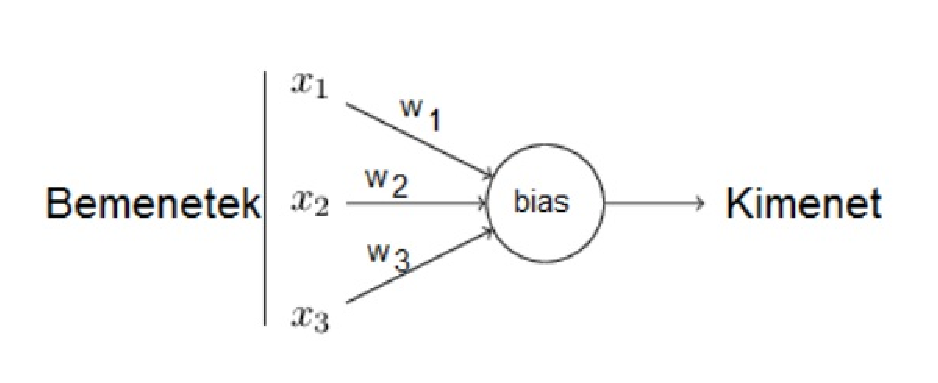
\includegraphics[scale=1]{images/neuron}
\caption{Sigmoid neuron}

\label{fig:neuron}
\end{figure}

Mindegyik bemenethez súlyok vannak rendelve, ami azt jelképezi, hogy az illető bemenet mennyire játszik fontos szerepet a neuron kimenetében. Minden neuronhoz tartozik továbbá egy "bias" ami a kisebb rendellenességek javítására szolgál.

A sigmoid neuron kimenete a \ref{eq:1} képlettel számítható ki.

\begin{equation} \label{eq:1}
\sigma(\sum\limits_{i=1}^{n-1} w_{i}*x_{i} + b)
\end{equation}

\begin{equation} \label{eq:2}
\sigma(z) = \frac{1}{1+e^{-z}}
\end{equation}

A \ref{eq:2} függvényt aktiválási függvénynek nevezik. Az aktiválási függvény szerepe, hogy a kimenetet egy adott intervallumba szorítsa. Ahogy ez a \ref{fig:sigmoidf} ábrán is látszik, a sigmoid neuron esetében ez az intervallum 0 és 1 között van. 

\begin{figure}[h]
\centering

\includegraphics[scale=1]{images/sigmoidf}
\caption{Szigmoid függvény grafikus képe}

\label{fig:sigmoidf}
\end{figure}

A szigmoid neuron egyik tulajdonsága, hogy kis változás a súlyokban, kis változást eredményez a kimenetben. Ez legalább annyira előny is, mint hátrány. Előny, mert amikor a kimenet közel van az elvárt kimenethez, a módosítások nem eredményezik azt, hogy a kimenet túlságosan eltávolodjon az elvárttól. Hátrány, mert amikor a kimenet nagyon helytelen, mint például a tanulás elején, hosszú időbe telik a javítása.

\begin{figure}[h]
\centering

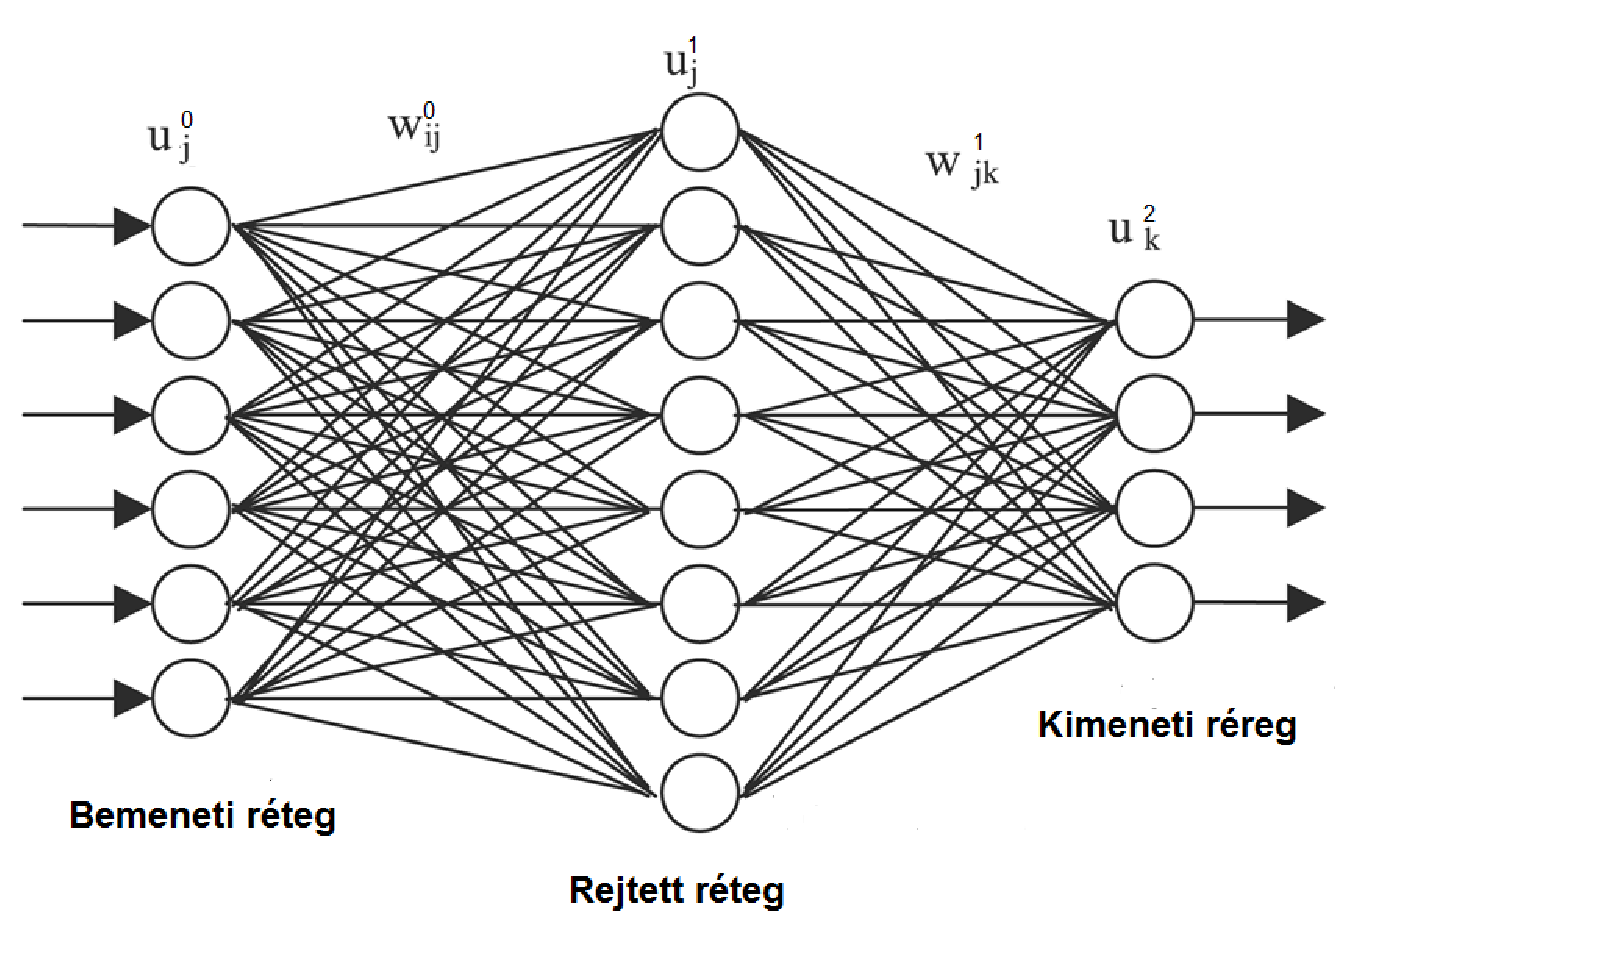
\includegraphics[scale=0.5]{images/net}
\caption{Egyszerű neurális háló}

\label{fig:net}
\end{figure}

A \ref{fig:net} ábrán egy egyszerű szigmoid neuronokból álló neurális háló látható. A súlyvektorok mérete már ennél a kis példánál is viszonylag nagy, ezért egy nagy hálónál ezek az értékek jelentősen megnőnek.


\section{Szerkezek}\label{sec:INTRO:architecture}

Olyan neurális hálót használtam, amelynek 625 bemenete és 43 kimenete van. A bemeneti neuronok a kép egy pixelének szürke árnyalatát tartalmazzák. A kimenetek száma megegyezik a forgalmi táblák osztályainak a számával. Különböző számú rejtett réteggel kísérleteztem, és ezeken belül is változó számú neuronnal.

\section{Sztochasztikus gradiens csökkentés}\label{sec:INTRO:graddesc}

Annak érdekében, hogy a súlyokat és bias-okat a kimenetnek az elvárt eredménytől való eltérése függvényében tudjam módosítani, a sztochasztikus gradiens csökkentést alkalmaztam. Ez a gradiens csökkentés egyszerűsített változata. Gradiens csökkentéssel a teljes tanítási adathalmazra számolja a hiba értékét, míg a sztochasztikus gradiens csökkentés közelíti a hibát egy bizonyos számú véletlenszerűen kiválasztott adat alapján. Minél nagyobb ez a szám, a közelítés pontossága annyival jobb lesz, de mivel nem a teljes adathalmazzal dolgozik, ezért gyorsabb lesz.

A \ref{eq:3} egyenlet a négyzetes hibafüggvény. \textit{n} a bemeneti tanítási adatok száma, \textit{y(x)} az \textit{x} bemenetre a háló által generált kimenet és \textit{a} az elvárt kimenet az \textit{x} bemenetre. Amikor az elvárt és a kiszámított kimenet közel van egymáshoz, a hiba kicsi lesz. Mivel a célom, hogy a kiszámított kimenet az elvárt kimenetet közelítse meg minél jobban, ezt a hibát kell minimalizálnom. Ennek érdekében bevezetem a  $\nabla C$-vel jelölt gradiensét a hibafüggvénynek. A gradiens értékét a \ref{eq:6} képlettel lehet kiszámítani.

\begin{equation} \label{eq:3}
\ C = \frac{1}{2n}\sum\nolimits_{x} \|y(x)-a(x)\|^2
\end{equation}

\begin{equation} \label{eq:6}
\ \nabla C = (\frac{\partial C}{\partial w_{i}},\frac{\partial C}{\partial b_{j}})^T
\end{equation}

A hiba csökkentése érdekében ismételtem alkalmaztam a \ref{eq:4} és a \ref{eq:5} szabályokat a súlyokra és bias-okra. $\eta$ a tanítási ráta. Ez egy kicsi érték kell legyen, de nem túl kicsi, mert akkor a tanulási folyamat túl lassú lenne.

\begin{equation} \label{eq:4}
\ w_{i} \rightarrow w_{i} - \eta\frac{\partial C}{\partial w_{i}} 
\end{equation}

\begin{equation} \label{eq:5}
\ b_{j} \rightarrow b_{j} - \eta\frac{\partial C}{\partial b_{j}} 
\end{equation}


\section{Backpropagation}\label{sec:INTRO:backprop}


A backpropagation algoritmus arra szolgál, hogy a háló súlyait és bias-ait úgy állítsa be, hogy a kimenet megközelítse minél jobban az elvárt kimenetet.

A \ref{eq:7} egyenletben $z^l$ a súlyozott bementi vektor az l-edik rétegben. Ahogy a \ref{eq:8} egyenletben látható, a kimeneti vektor egy rétegben az előző réteg kimenetének használatával számolható ki, vagyis az információ továbbításával. A háló kimenetének kiszámítása után a \ref{eq:9}-es egyenlet segítségével lehet kiszámolni az utolsó réteg hibáját, ahol \textit{L} a rétegek számát jelöli, \textit{$\nabla_aC$} pedig a $\frac{\partial C}{\partial a_j^L}$ parciális deriváltakat tartalmazó vektor.


Maga a backpropagation a \ref{eq:10} képlet segítségével történik minden \textit{l} rétegre, \textit{L-1}-től 2-ig.

\begin{equation} \label{eq:7}
\ z^l = (w^l*a^{l-1} + b^l) 
\end{equation}

\begin{equation} \label{eq:8}
\ a^l = \sigma(z^l) 
\end{equation}

\begin{equation} \label{eq:9}
\ \delta^L = \nabla_aC \circ \sigma'(z^L)
\end{equation}

\begin{equation} \label{eq:10}
\ \delta^l = ((w^{l+1})^T* \delta^{l+1}) \circ \sigma'(z^l)
\end{equation}

\chapter{Az algoritmus} \label{algorihm}

\begin{enumerate}
   \item Súlyok és bias-ok inicializálása véletlenszerű adatokkal
   \item Minden ciklusra végezd:
   \begin{enumerate}
   		\item Tanulási adatok összekeverése
   		\item Minden batch-re végezd:
   		\begin{enumerate}  %updateMinibatch
   			\item Minden tanulási adatra a batch-ből végezd:
			    \begin{enumerate}
			      \item Mindegyik neuron kimenetének a kiszámítása a bemenettől a kimenet felé
			      \item Kimenet hibájának kiszámítása
		    	  \item Minden neuron hibájának kiszámítása a kimenettől a bemenet felé haladva
			    \end{enumerate}
		    \item Gradiens csökkentés: súlyok és bias-ok újraszámolása 
   		\end{enumerate}
   \end{enumerate}
   
 \end{enumerate}
 
 Ahhoz, hogy a háló tanulni tudjon, fontos az, hogy a súlyokat és bias-okat megfelelően kicsi számokkal inicializáljuk. Ezt úgy valósítottam meg, hogy a 0 és 1 között véletlenszerűen generált számot elosztottam 3000-el.
 
 A batch-ben egyidőben jelen levő adatok minél változatosabbak kell legyenek, annak érdekében hogy tanulás közben egy időben figyelembe vegye a különböző osztályok tulajdonságait. Ezért van szükség az adatok összekeverésére. A beolvasás sorban történik, vagyis az azonos osztályba tartozóak egymás után fognak szerepelni. Ha ebben a sorrendben kerülnének be a batch-be, akkor a háló először megpróbálná megtanulni az egyik osztály tulajdonságait, utána pedig sorban a következőkét. Az adatok keverésével ezt kerülöm el. \cite{5}